%%%%%%%%%%%%%%%%%%%%%%%%%%%%%%%%%%%%%%%%%%%%%%%%%%%%%%%%%%%%%%%%%%%%%%%%%%%%%%%%%
\section{Inleiding}
\emph{Redirected walking} is een techniek waarbij een proefpersoon in een 
virtuele omgeving weergegeven in een head-mounted display kan rondwandelen door 
middel van het vervormen van de route die deze proefpersoon in een fysieke 
omgeving wandelt. Het doel is, door de 1:1 relatie van fysieke beweging en 
virtuele beweging te ontkoppelen, rondwandelen in grotere tot zelfs arbitrair 
grote virtuele ruimtes mogelijk te maken. Ik zal diverse technieken bespreken die
gebruikt worden om deze ontkoppeling teweeg te brengen. Naast de
redirectietechnieken zijn er ook technieken die de immersie verbeteren door
andere zintuigen te betrekken bij het proces.

%%%%%%%%%%%%%%%%%%%%%%%%%%%%%%%%%%%%%%%%%%%%%%%%%%%%%%%%%%%%%%%%%%%%%%%%%%%%%%%%%
\section{Redirectietechnieken (RDTs)}
RDTs zijn technieken waar de fysieke bewegingen van een proefpersoon ontkoppeld
worden van de resulterende virtuele bewegingen. Dit kan bijvoorbeeld gebeuren 
door de snelheid van de proefpersoon in de virtuele omgeving te versnellen of te
vertragen ten opzichte van de snelheid in de fysieke omgeving, of door de
rotaties te vertragen of te versnellen zodat de proefpersoon het tracking gebied
niet verlaat. Ik beschrijf hier kort enkele van deze technieken samen met 
onderzoeken die er over gevoerd zijn.


\subsection{Rotationele vervorming}
Bij rotationele vervorming worden de rotaties van de proefpersoon in de 
virtuele omgeving vertraagd of versneld ten opzichte van de rotaties in de
fysieke omgeving, een voorbeeld hiervan kan men zien in Figuur 
\ref{fig:kohn01-movement}. In het algemeen is het hier het doel om de
proefpersoon indien mogelijk steeds richting het midden van de tracking area
te doen wandelen.

\begin{figure}[h!]
    \centering
    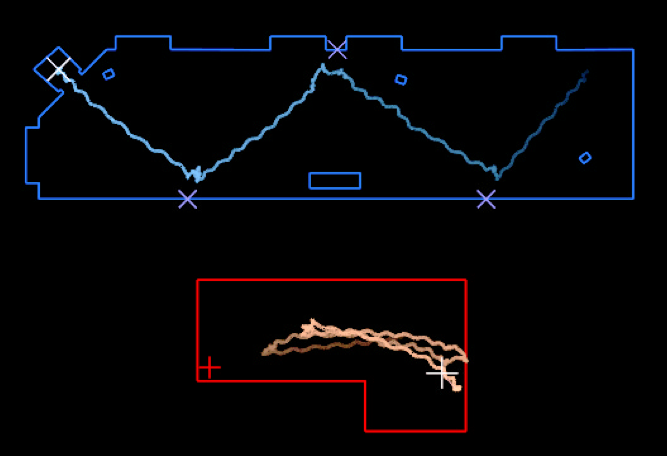
\includegraphics[width=0.7\textwidth]{kohn01-movement}
    \caption{Vergelijking van de beweging van de proefpersoon in de virtuele
    omgeving (blauw) en de overeenkomstige beweging in de fysieke omgeving 
    (rood).\cite{kohn01}}
    \label{fig:kohn01-movement}
\end{figure}

Deze techniek is al in diverse papers onderzocht:

In een onderzoek gevoerd door Razzaque et. al., 2001 \cite{kohn01} werden 
proefpersonen gevraagd om een virtuele brandoefening uit te voeren. In de 
opstelling voor dit onderzoek waren er in het fysieke labo twee knoppen geplaatst
op dezelfde afstand als in de virtuele omgeving. In de virtuele omgeving waren er
echter 4 knoppen met telkens een hoek van 90 graden er tussen, deze opstelling is
in bovenaanzicht getoond in Figuur \ref{fig:kohn01-movement}. In dit onderzoek
werd op enkele verschillende manieren rotationele vervorming ingevoegd:

Als de proefpersoon stilstaat werd er een kleine hoeveelheid ``drift'' 
toegevoegd, de camera in de virtuele omgeving draaide automatisch zeer traag in 
de omgekeerde richting van waar men de proefpersoon in de fysieke omgeving heen 
wilde naar laten kijken. Het bleek dat de proefpersoon hierdoor automatisch in
die richting ging draaien om het beeld stil te houden. De rotaties van de
proefpersoon werden ook overdreven, of juist gedempt, om de proefpersoon in de
fysieke omgeving in de juiste richting te laten wandelen.

Naast deze vervormingen indien de testpersoon in stilstand was, was het ook
mogelijk om een schijnbaar rechte lijn in de virtuele omgeving overeen te laten
komen met een curve. Dit effect werd bekomen door het pad in de virtuele omgeving
een bepaalde hoeveelheid te buigen, proportioneel met de lineaire snelheid van
de proefpersoon in de fysieke omgeving.

Een combinatie van deze methodes werd gebruikt om er voor te zorgen dat als de
proefpersoon in de fysieke omgeving voor een knop stond, dit in de virtuele
omgeving ook het geval was. Helaas was het voor deze implementatie nodig dat er
een voorberekend pad door de virtuele omgeving bestond, en dat de proefpersoon
er zo weinig mogelijk van afweek. Later werden er technieken voorgesteld om deze
vereisten te verzwakken.

In Engel et. al., 2008 \cite{engel08} wordt een techniek voorgesteld om deze 
rotationele vervorming dynamisch te bepalen. Dit werd gedaan door het 
dynamische-rotatie probleem te reduceren tot een optimisatie probleem, welke in 
de AI gemeenschap reeds bekend zijn. Dit algoritme maakte het mogelijk om 
optimale rotationele vervormingen te berekenen maar vereist in ieder geval een 
gedeeltelijke kennis over het te volgen virtuele pad, en vereist dat het pad een
bepaalde hoeveelheid bochten bevat.

In een ander onderzoek in Neth et. al., 2012 \cite{neth12} werd verder 
onderzocht wat de precieze relatie tussen bewegingssnelheid en maximaal 
acceptabele rotationele vervorming is. Uit dit onderzoek bleek dat tragere 
snelheden grotere vervormingen toelaten, maar dat deze relatie niet lineair is.
Aangezien mensen over het algemeen trager wandelen in virtuele omgevingen
\cite{mohler07}, kan men dit toepassen in redirected walking.

In een tweede experiment uit hetzelfde onderzoek \cite{neth12} werd onderzocht 
of deze bevindingen effectief konden gebruikt worden dynamische schalering van 
vervorming toe te passen in een rijke virtuele omgeving. Er werd hier onderzocht 
of er een significant verschil is tussen de merkbaarheid van statische 
rotationele vervorming (als de proefpersoon stil staat) versus dynamische 
rotationele vervorming (als de proefpersoon beweegt). Naast de technieken van 
Razzaque et. al., 2001 \cite{kohn01} om rotationele vervorming in te voegen met 
een constant, een statisch en een dynamisch component, werd er ook gebruik 
gemaakt van versterking van de effecten nabij de randen van de fysieke omgeving, 
om het verlaten van het tracking gebied te vermijden. Er werd gemeten wat de 
mediaanafstand is die een proefpersoon kan wandelen in een grote virtuele 
omgeving voor de proefpersoon moet geforceerd geherori\"enteeerd worden richting
het centrum van de fysieke omgeving om het verlaten van het tracking gebied te 
voorkomen. Uit dit experiment is gebleken dat er een positief significant 
verschil is tussen de mediaan gewandelde afstand bij dynamische vervorming 
versus statische vervorming zonder een significante verhoging in simulatorziekte.

Uit al deze onderzoeken blijkt dat er een trade-off is tussen een virtuele 
omgeving met een ongekend pad\cite{neth12} versus een betere immersie wegens 
minder onderbrekingen\cite{engel08,kohn01}. 

Alle vorige studies behandelden rotationele vervorming in beweging, dus over 
curves. Het is echter ook mogelijk om rotationele vervorming in stilstand te
hebben. In Steinicke et. al., 2009 \cite{steinicke09} werd bepaald dat in dit 
specifieke geval compressies tot 77\% acceptabel zijn voor de proefpersoon het 
merkt.


\subsection{Translationele vervorming}
Naast rotationele vervorming is het ook mogelijk om de lineaire snelheid van een
proefpersoon te vervormen daar onderzoek heeft aangetoond dat proefpersonen in 
virtuele omgevingen afstand \cite{loomis03}, snelheid \cite{banton05} en 
afgelegde afstand \cite{frenz07} onderschatten. In Steinicke et. al., 2009 \cite{steinicke09} 
werd er een experiment uitgevoerd om onder andere te bepalen wat de maximaal 
acceptabele translationele vervorming is voor een gegeven snelheid. Er werd 
bepaald dat de vervorming merkbaar is bij een versnelling tussen 20\% en 60\% 
met een ideale waarde van ongeveer 20\%.

Rotationele vervorming en translationele vervorming vormen de basis van
redirected walking, en zijn ook de twee technieken die gebruik maken van
ontkoppeling van het fysieke en het virtuele pad van de proefpersoon.


\subsection{Change blindness}
Change blindness slaat op de manier waarop mensen onder bepaalde omstandigheden
verrassend grote veranderingen in een omgeving niet merken. In een paper van
Simons et. al., 2005 \cite{simons05} wordt er een breed overzicht gegeven van de
diverse experimenten die zijn uitgevoerd rond dit fenomeen. Zo merken veel mensen
bijvoorbeeld helemaal niet als een persoon in het midden van een interactie door
een totaal andere persoon wordt vervangen\cite{simons98}, of wordt het verschil
tussen twee foto's die om de beurt worden getoond pas na een zeer lange tijd
opgemerkt\cite{rensink97}.

Omdat dit zo een krachtig fenomeen is, wordt het ook toegepast in redirected 
walking. Waar de vorige technieken het fysieke en het virtuele pad van de 
proefpersoon ontknoppelden probeert deze techniek de proefpersoon te misleiden, 
en er voor te zorgen dat hij in de tracking ruimte blijft door de layout van de 
virtuele omgeving strategisch aan te passen, bijvoorbeeld door een deur van
plaats te laten wisselen zoals in Figuur \ref{fig:suma1}.

\begin{figure}[h!]
    \centering
    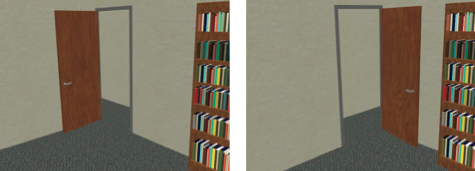
\includegraphics[width=0.7\textwidth]{suma1}
    \caption{Voorbeeld van een verandering in een virtuele omgeving.\cite{suma11}}
    \label{fig:suma1}
\end{figure}

In Suma et. al., 2011 \cite{suma11} werd er getest of veranderingen in de 
virtuele omgeving voor de proefpersonen merkbaar waren. De proefpersoon werd
gevraagd om in een virtueel kantoor in elke kamer een beeldscherm uit te zetten
en vervolgens de kamer verlaten. Dit proces werd dan herhaald voor 16 kamers.
Nadat het beeldscherm werd uitgezet veranderde de deur van positie zodat de gang
in een hoek van 90 graden verder ging ten opzichte van hoe de proefpersoon de
kamer binnenkwam. Dit hele proces is zichtbaar in Figuur \ref{fig:suma2}.

\begin{figure}[h!]
    \centering
    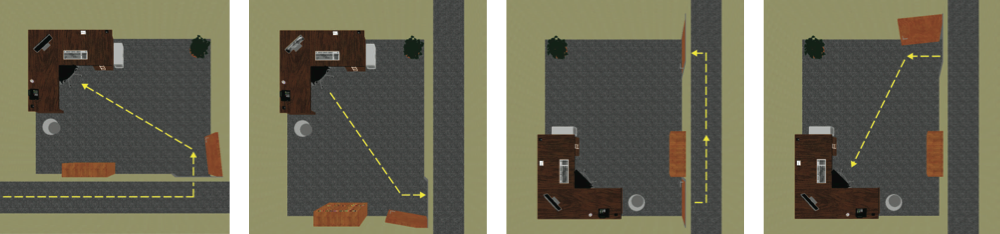
\includegraphics[width=\textwidth]{suma2}
    \caption{Verandering van de positie van de deur in het onderzoek van Suma et. 
    al., 2011 \cite{suma11}.}
    \label{fig:suma2}
\end{figure}

Door de veranderingen van de fysieke omgeving op deze manier te laten gebeuren
werd de proefpersoon geforceerd cirkels rond de tracking area te wandelen, in
Figuur \ref{fig:suma3} is een illustratie van het pad door een kamer te zien.

\begin{figure}[h!]
    \centering
    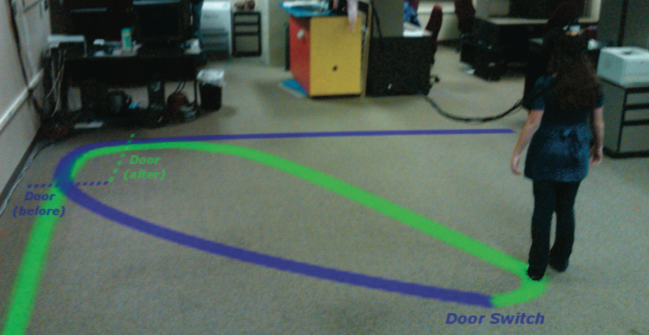
\includegraphics[width=0.7\textwidth]{suma3}
    \caption{Voorbeeld van een verandering in een virtuele omgeving.\cite{suma11}}
    \label{fig:suma3}
\end{figure}

Uit de afgenomen vragenlijst is toen gemerkt dat deze verandering voor bijna 
iedereen compleet onmerkbaar was, en werd er zelfs maar in kleine mate ervaren
dat men in cirkels was aan het wandelen.


\subsection{Afleiders}
Een laatste techniek die ik zal bespreken is het toevoegen van ``afleiders'',
dynamisch bewegende voorwerpen of personen die als doel hebben de proefpersoon
uit eigen wil zijn pad te laten afbuigen. Afleiders kunnen ook gebruikt worden
om de ontkoppelingen van het virtuele en het fysieke pad minder te laten 
opvallen.

In een onderzoek van Neth et. al., 2012 \cite{neth12} werd er bijvoorbeeld 
gebruik gemaakt van andere virtuele avatars zoals in Figuur \ref{fig:avatars}.
Er werd gebruik gemaakt van avatars die recht voor de proefpersoon gingen
stilstaan om deze af te dwingen te vertragen indien hij te snel ging om het pad
effectief af te buigen. Er werd ook gebruik gemaakt van avatars die op koers
wandelden voor een botsing om de proefpersoon te forceren af te buigen.

\begin{figure}[h!]
    \centering
    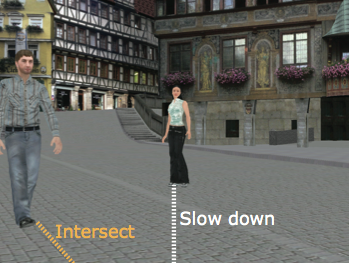
\includegraphics[width=0.7\textwidth]{avatars}
    \caption{Voorbeeld van avatars in een virtuele omgeving, met als doel de
    proefpersoon te laten vertragen of zijn pad af te buigen.\cite{neth12}}
    \label{fig:avatars}
\end{figure}

In Peck et. al., 2009 \cite{peck09} werd er op een andere manier gebruik gemaakt 
van afleiders. Er werd gevraagd aan de proefpersoon om een vlinder te volgen om
hem de illusie te geven dat hij \mbox{360\textdegree} heeft gedraaid terwijl hij 
eigenlijk maar 180\textdegree{} heeft gedraaid. Hieruit bleek dat proefpersonen 
minder het gevoel hadden dat de wereld versneld draaide met een afleiding dan 
bij andere technieken.


%%%%%%%%%%%%%%%%%%%%%%%%%%%%%%%%%%%%%%%%%%%%%%%%%%%%%%%%%%%%%%%%%%%%%%%%%%%%%%%%%
\section{Reori\"entatietechnieken (ROTs)}
Hoewel redirectietechnieken bedoeld zijn om een proefpersoon binnen een tracking
area te laten wandelen, kan het soms gebeuren dat een botsing met de rand van de
tracking area niet meer te vermeiden is. Als dit het geval is wordt er gebruik
gemaakt van ``reori\"entatietechnieken''. Dit zijn directe commando's aan de
proefpersoon om van koers te veranderen, en vallen daarom ook behoorlijk op. Ik
beschrijf hier de meest voorkomende ROTs.


\subsection{Verbale commandos}
Bij verbale commandos wordt er een geluidssignaal gegeven (meestal een gesproken
signaal) waarin de proefpersoon wordt gevraagd om te draaien.

In het onderzoek van Razzaque et. al., 2001 \cite{kohn01} werd, indien de
proefpersoon dreigde het tracking gebied te verlaten, de proefpersoon met verbale
commando's gevraagd stil te staan en heen en weer te kijken om de proefpersoon in
de fysieke omgeving terug in de juiste richting te laten kijken.

Er werd in een andere studie van Peck et. al., 2009 \cite{peck09} echter bevonden 
dat verbale commando's niet de beste optie zijn voor redirectietechnieken, omdat
deze makkelijk genegeerd kunnen worden.


\subsection{Visuele commandos}
Bij visuele commandos wordt er een signaal op de display weergegeven om de 
proefpersoon te vragen om te draaien.

In het onderzoek van Neth et. al., 2012 \cite{neth12} werd onder andere gebruik 
gemaakt van een stopteken. Als dit werd getoond werd de hele virtuele wereld stil 
gelegd. Er werd op voorhand aan de proefpersoon gevraagd rond te draaien tot het 
stopteken verdwijnt indien het getoond werd. Hoewel dit een zeer intrusieve 
methode is, is ze zeer effectief om het verlaten van het tracking gebied te 
voorkomen daar ze niet te negeren is.


%%%%%%%%%%%%%%%%%%%%%%%%%%%%%%%%%%%%%%%%%%%%%%%%%%%%%%%%%%%%%%%%%%%%%%%%%%%%%%%%%
\section{Immersie}
Hoewel visie voor redirected walking het belangrijkst is, omdat bij conflicten
tussen het proprioceptieve\footnote{Het zintuig dat de relatieve afstand tussen
lichaamsdelen waarneemt.} en het vestibulaire\footnote{Het zintuig 
verantwoordelijk voor ons evenwichtsgevoel.} systeem en visie, visie vaak dit
conflict wint\cite{berthoz02,dichgans78,bruder08}, zijn de andere zintuigen toch
belangrijk om immersie te verkrijgen. Als men in een virtuele omgevingen geluid 
realistisch kan positioneel reproduceren helpt dit bijvoorbeeld de immersie 
enorm\cite{lackner77}, maar zelfs het maskeren van geluid van in de fysieke 
wereld met bijvoorbeeld ruis kan helpen\cite{usoh99}.

In Engel et. al., 2008\cite{engel08} wordt ook opgemerkt dat de hoeveelheid 
omgevingslicht en omgevingsgeluid dat binnensijpelt een merkbare negatieve 
invloed heeft op de effectiviteit van redirectietechnieken. Naast audio is het 
ook mogelijk om de immersie te verhogen met proxy-objecten in de fysieke 
omgeving die overeen komen met objecten in de virtuele omgeving\cite{steinicke09}
zoals te zien is in Figuur \ref{fig:proxy-object}.

\begin{figure}[h!]
    \centering
    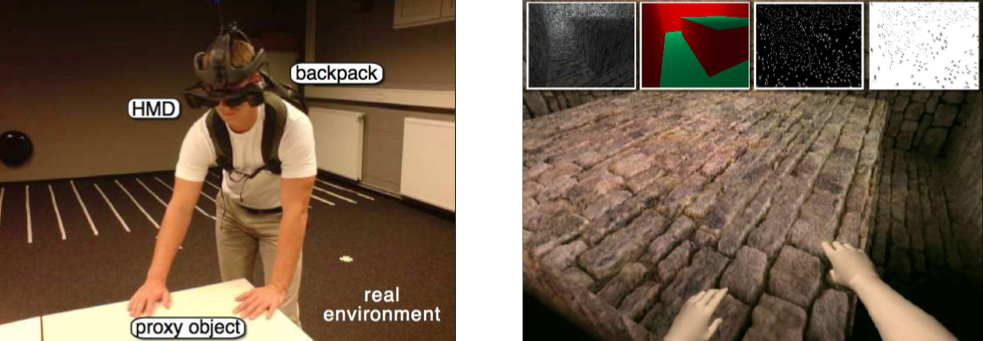
\includegraphics[width=0.7\textwidth]{proxy-object}
    \caption{Voorbeeld van een proxy-object en het overeenkomstige beeld dat de
    proefpersoon ziet.\cite{steinicke09}}
    \label{fig:proxy-object}
\end{figure}

Voor de effectieve weergave van de virtuele omgeving maakt men meestal gebruik 
van een head mounted display, of een HMD. Voor HMDs is het ideaal om een zo hoog 
mogelijke field of view te hebben, dit lijkt geen groot effect te hebben op de 
prevalentie van simulatieziekte\cite{arthur00} maar verhoogt de performantie en 
immersie drastisch\cite{arthur00}.

Traditioneel waren HMDs met grote field of view zeer duur en niet beschikbaar voor
consumenten, maar tegenwoordig zijn er enkele betaalbare HMDs beschikbaar met een
redelijk grote field of view, zoals de Oculus Rift DK1 (110\textdegree{} 
diagonaal).

\begin{figure}[h!]
    \centering
    \includegraphics[width=0.7\textwidth]{or-dk1}
    \caption{De Oculus Rift Developer Kit 1}
    \label{fig:or-dk1}
\end{figure}

Ten laatste is het voor redirected walking ook belangrijk dat de positie van
de proefpersoon in de fysieke omgeving geweten is tot in grote precisie. Er zijn
hier echter een grote hoeveelheid commerci\"ele systemen voor beschikbaar zoals
het OptiTrack systeem. Ik ga hier niet verder op in.


%%%%%%%%%%%%%%%%%%%%%%%%%%%%%%%%%%%%%%%%%%%%%%%%%%%%%%%%%%%%%%%%%%%%%%%%%%%%%%%%%
\section{Conclusie}
De technieken voor redirected walking vari\"eren van technieken die een
ontkoppeling van de virtuele en fysieke omgeving verwezenlijken om een arbitrair
pad in de virtuele omgeving in de fysieke omgeving te laten passen, tot
technieken zoals change blindness die gebruik maken van eigenaardigheden van het
menselijk brein om de virtuele omgeving aan te passen zodat deze in de fysieke
omgeving past.

Hoewel redirected walking een realistische en immersieve omgeving kan cre\"eren 
zijn er toch enkele inherente zwaktes waar op zich niet omheen kan gewerkt 
worden. Zo is het bijvoorbeeld onmogelijk om arbitraire fysieke collisie overeen 
te laten komen met collisie in de virtuele omgeving tenzij het labo expliciet 
voor die virtuele omgeving is gebouwd. Het is ook niet mogelijk om de textuur van
de vloer in de fysieke omgeving overeen te laten komen met deze in de virtuele
omgeving als deze verandert van kamer tot kamer.

Ondanks deze relatief kleine beperkingen is redirected walking toch zeer
geschikt voor gebruik in toepassingen zoals virtuele rondleidingen, of het
doorlopen van een virtuele impressie van een huis voor het effectief gebouwd
zal worden.